
\section{ Experiment}

\noindent We used the map of Helsinki in our simulator to evaluate performance of the proposed ACP. We compare ACP with Binary Spray and Wait (BSW) protocol \cite{C31}, distributed social-based location privacy protocol (SLPD) \cite{C16} and our Multi-Hop Location-Privacy Protection (MHLPP). We simulated the continuous movement of users along streets on the map with one LBSP, fixed at a random location on the map.

For each user, we associate a random social value between 0 - 100\%, each corresponding to other users. Since each social value is assigned with equal probability, we can compute the expected number of friends of an user. If an user whose social value is larger than 85\% is called a friend and there are \textit{n} users in the network, then there are $n\times \left(1-85\%\right)$ friends for this user in consideration.

The Shortest Path Map-Based Movement (SPMBM) \cite{C35} is used in our experiment for the user mobility model. For each experiment, we give the simulator a random seed so that it can generate a pseudo-random number based on the seed. Therefore, all the factors including users' speed and locations are the same if two experiments have the same random seed. All four protocols are tested using the same set of random seeds.

Before each experiment, the simulator runs for 800 seconds, and then we pick 100 users out of 126 users randomly to send a query to the LBSP. The simulation then lasts for 20 minutes before we measure different parameters for performance analysis. 


\subsection{ Average Query Success Ratio}

\noindent The query success ratio is the percentage of delivered queries among some attempts. Since users sending 100 queries in each experiment, if $s$ queries are delivered to the LBSP at time $t$, the query success ratio of time $t$ is $s\%$.

As shown in Figure \ref{fig:AverageQuerySuccessRatio10}, we compare the average query success ratio of the four protocols for 5 different communication ranges (10, 30, 50, 70 and 90 meters) at 10 minutes mark. We observe that our ACP and BSW achieve high query success ratio, while the query success ratio in case of MHLPP and SLPD are lower than the other two. BSW has the highest query success ratio because it is a no-privacy protocol. The ACP has slightly lower query success ratio than BSW, because the query delivery process of the ACP is almost the same as that of BSW. Since users of ACP must wait for available ACs, it requires more time to initiate their queries. However, ACP and BSW exhibit similar performance compared to the other two protocols. MHLPP and SLPD need to find friends to obfuscate their queries, which complicates their query delivery process.

\begin{figure} [htbp]
\centering 
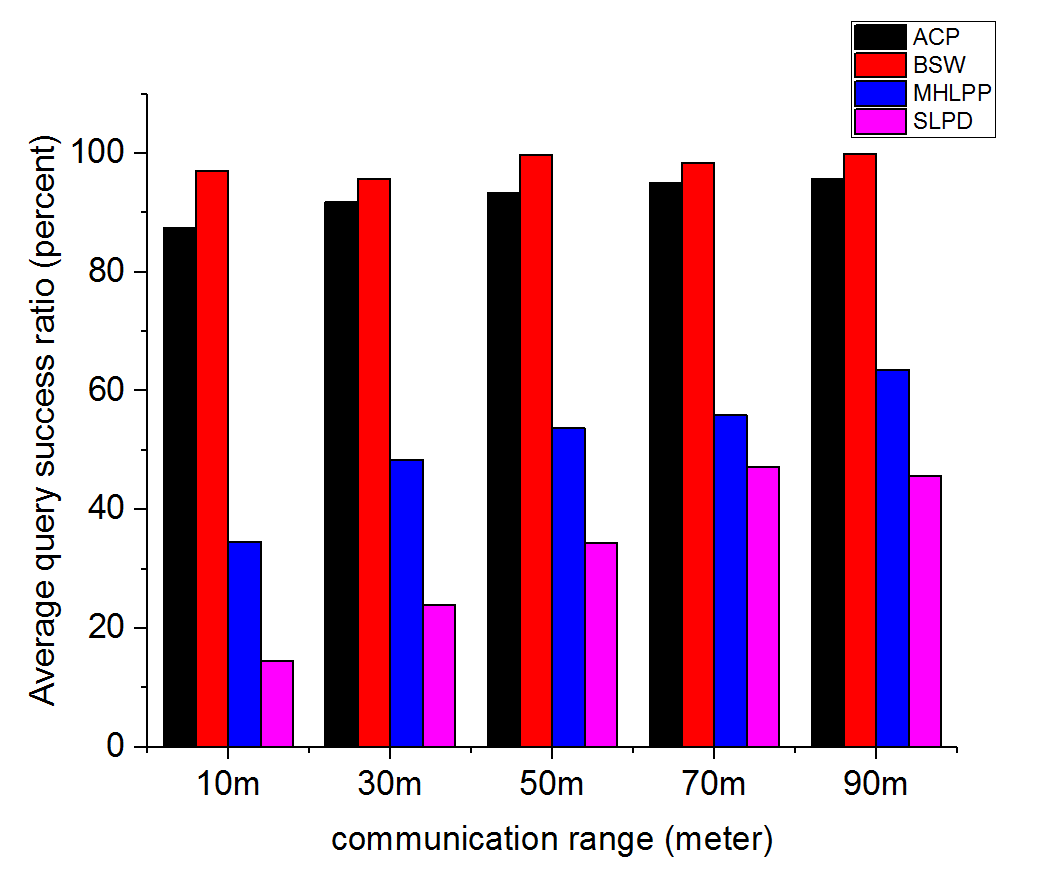
\includegraphics[width=4.0in]{olgraph/QsrCr.png}
\caption{Average Query Success Ratio (at 10 minutes mark)} 
\label{fig:AverageQuerySuccessRatio10} %% label for entire figure 
\end{figure}

The results at 20 minutes mark is shown in Figure \ref{fig:AverageQuerySuccessRatio20}. Both MHLPP and SLPD give much higher query success ratio after 20 minutes than after 10 minutes. That is because they require more time in their obfuscation phases when they need to find friends. In fact, some of the queries of MHLPP and SLPD still do not finish their obfuscation phase at 20 minutes mark.

\begin{figure} [H]
\centering 
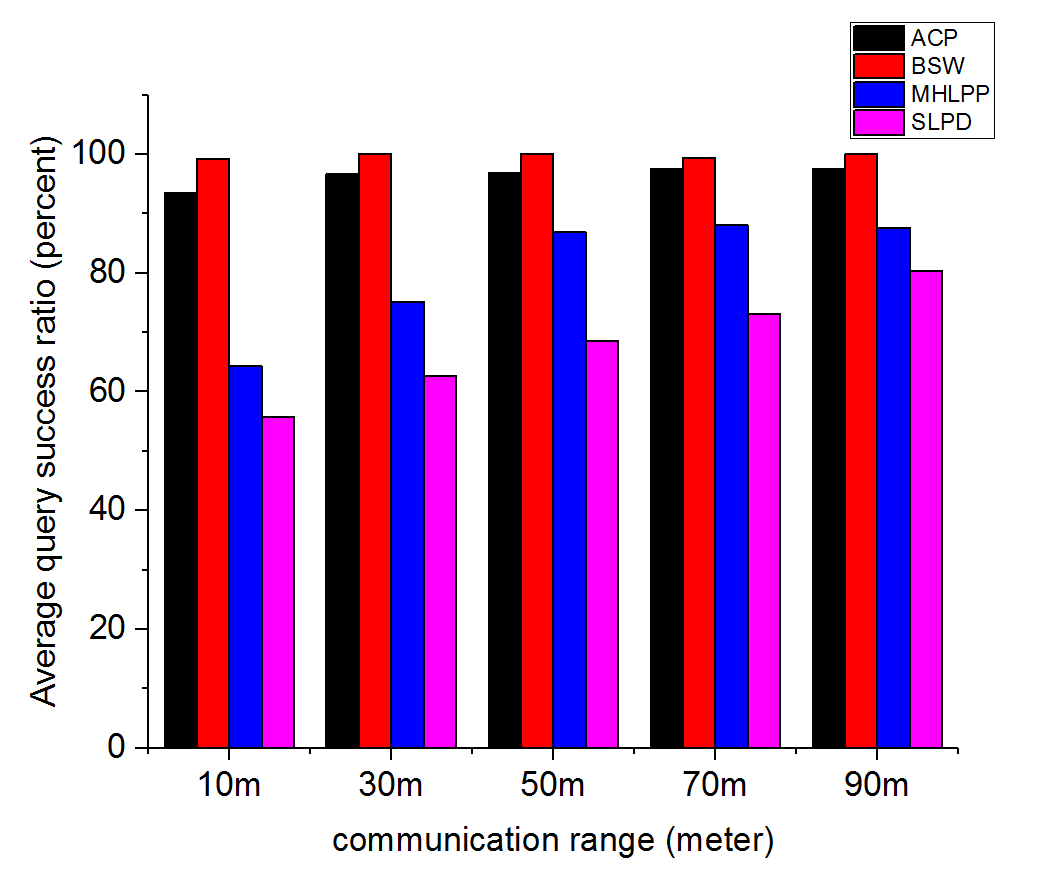
\includegraphics[width=4.0in]{olgraph/QsrCr20.png}
\caption{Average Query Success Ratio (at 20 minutes mark)} 
\label{fig:AverageQuerySuccessRatio20} %% label for entire figure 
\end{figure}

The communication range can influence the query success ratio. In most of the cases, the success ratio rises when we increase the communication range, and its influence is especially evident under 50 meters. A large communication range makes it easy for users to encounter others, which is good for them to forward queries. However, an user who is so far away from the destination does not want the intermediates of his query encounters many users nearby. Because all users who carry copies of that query are near the sender instead of the destination, which decreases their query success ratio. Therefore, when the communication range reaches 70 meters, the success ratios almost stay flat.

In Figure \ref{fig:F416AverageQuerySuccessRatioWith50MetersCommunicationRatio}, we observe that both ACP and BSW have better convergence speed than MHLPP and SLPD. In other words, the former two protocols approach the 100\% query success ratio mark faster than the latter two. At the very beginning, the ACP even has a little higher query success ratio than BSW. Because the ACP users need ready AC, and most of the users get their first \textit{ready}-ACs at places where there are many users, users rarely generate query near the edges of the map at the beginning, which facilitates their queries delivery process. For example, if an user generates his query at the edge of the map, the copies of this query might be sent to users who are also at the edge, and it takes more time for them to deliver the query. If the user does not generate his query until he arrives at a place near the center, the copies of this query will be carried by the users in the center with higher probability.

\begin{figure} [hbtp]
\centering 
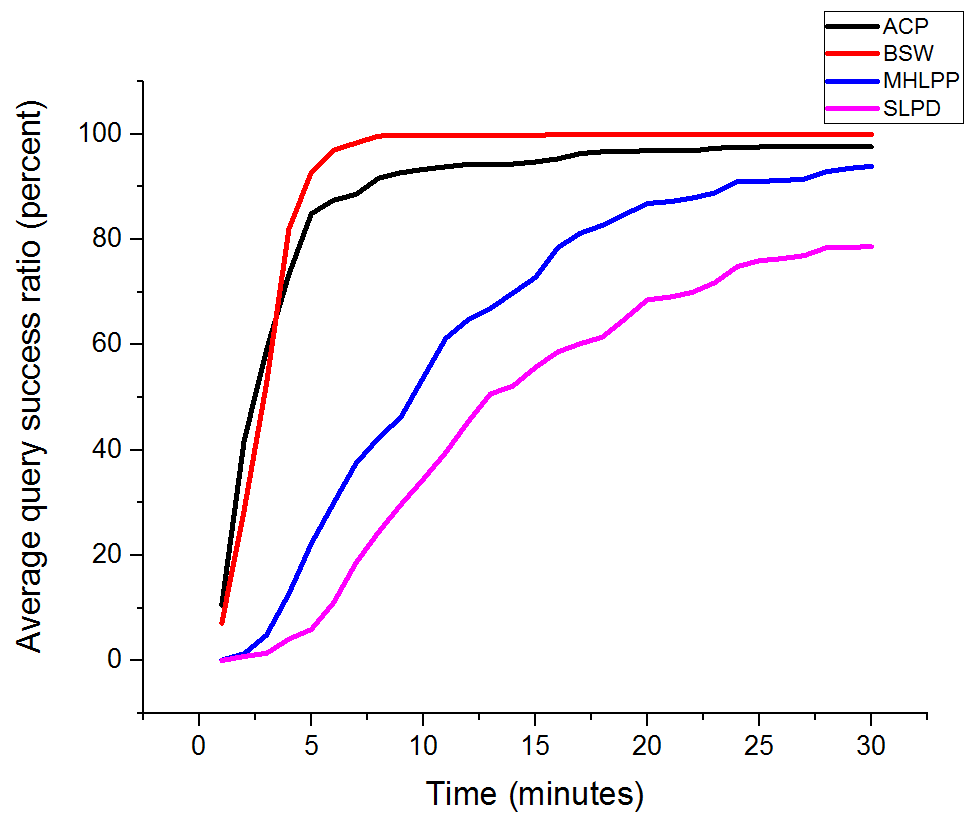
\includegraphics[width=4.0in]{figures/F416AverageQuerySuccessRatioWith50MetersCommunicationRatio.png}
\caption{Average Query Success Ratio for 50-Meters Communication Range} 
\label{fig:F416AverageQuerySuccessRatioWith50MetersCommunicationRatio} %% label for entire figure 
\end{figure}

\subsection{ Average Reply Success Ratio}

\noindent When the LBSP receives a query, it sends a reply to the requester. If the reply reaches the original requester before the test ends, we view it as a success; otherwise, the reply is considered to be failed. There are three reasons for not receiving reply: 1) the query is not delivered to the LBSP successfully; 2) the query took too much time for which the reply could not be delivered in time; or 3) the route of the reply is too long. Since there are 100 queries in each experiment, we expect the number of replies should be 100. 

In Figure \ref{fig:F417AverageReplySuccessRatioWith50MetersCommunicationRatio}, the BSW has a significantly higher reply success ratio than all other protocols, because it is a no-privacy protocol. ACP has a higher ratio than MHLPP and SLPD, but its advantage is not as large as that in the query process. In fact, the reply process of MHLPP and SLPD are simpler than that of the ACP, but the ACP saves much time in its query process so that it has a better reply success ratio than the other two.

\begin{figure} [hbtp]
\centering 
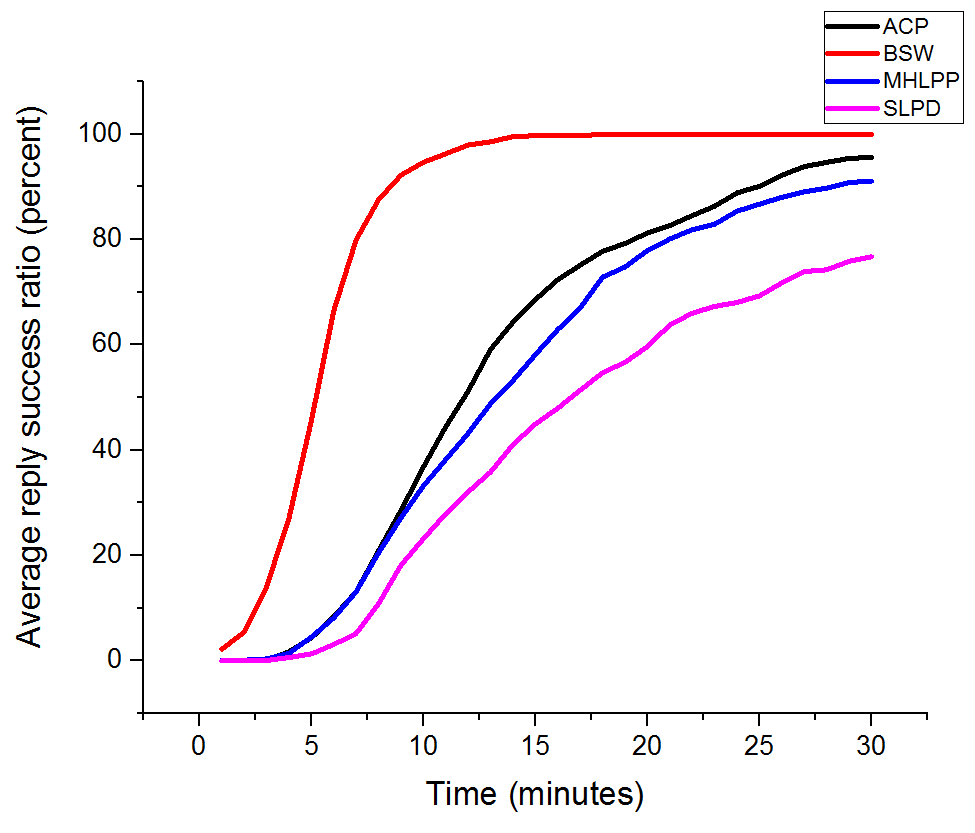
\includegraphics[width=4.0in]{figures/F417AverageReplySuccessRatioWith50MetersCommunicationRatio.png}
\caption{Average Reply Success Ratio for 50-Meters Communication Range} 
\label{fig:F417AverageReplySuccessRatioWith50MetersCommunicationRatio} %% label for entire figure 
\end{figure}

\subsection{ Total Number of Query Relays}

\noindent The query delivery process of all the four protocols use store and forward strategy, and BSW makes copies for queries and gives half of the copies to any users it encounters. That is a significant cost for the network, so we use the number of query relays (QR) to evaluate that cost. The QR is initialized as zero at the beginning of the test. When an user relays one or several copies of a query, we increase QR by 1. For example, in SLPD, there are two phases: the obfuscation phase and the free phase. In the obfuscation phase, a query is forwarded among one-hop friends for $k$ times. After that, it is forwarded using BSW protocol. BSW makes $c$ copies of the query and gives half of the copies to any encountering user. Thus, QR should be roughly $k+c$. Since the user gives all its copies to the destination at once if he encounters the destination, the QR may be smaller. The smaller that number is, the smaller the cost of the network is. Since there are 100 queries, we divide QR by 100 to get an average value. 

In Figure \ref{fig:F418AverageTotalNumberofForwardingQueriesAt20Minutes}, we compare QR in all four protocols. We observe that both BSW and ACP have slightly lower QR than the other two. In case of ACP and BSW, they deliver queries so fast that users who carry more than one copy give all their copies to the destination before they send these copies to different users separately. As a result, many copies have no chance to be forwarded, which decreases the cost. 

While both MHLPP and SLPD have obfuscation phases, the queries start to be delivered freely (as in BSW) at a random place which might be so far away from the destination, so that almost all copies can be forwarded.

\begin{figure} [hbtp]
\centering 
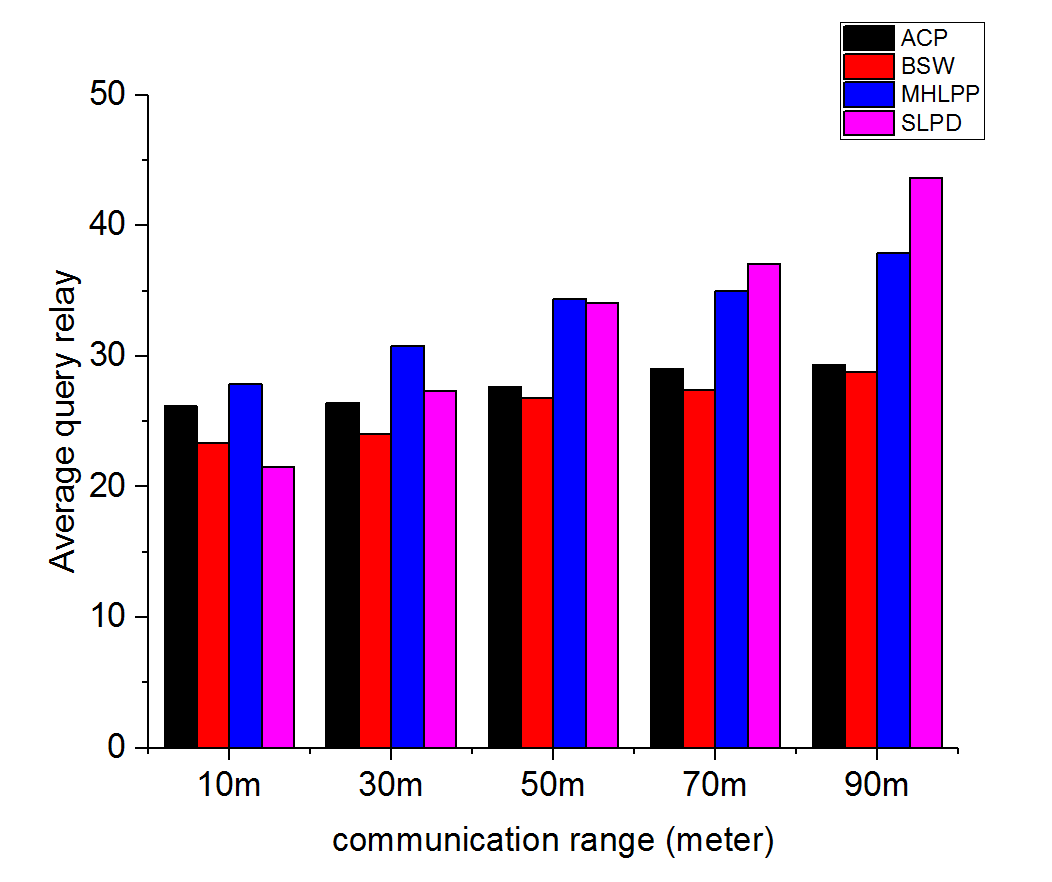
\includegraphics[width=4.0in]{olgraph/QrCr.png}
\caption{Average Number of Forwarding Queries At 20 Minutes Mark} 
\label{fig:F418AverageTotalNumberofForwardingQueriesAt20Minutes} %% label for entire figure 
\end{figure}

The communication range affects the total number of forwarding queries, especially in the case of MHLPP and SLPD. These two protocols can finish their obfuscation phase more quickly in a larger communication range scenario, so that more queries can be forwarded freely (as in BSW), which makes their QR larger.

\subsection{ Memory Cost}

\noindent We count the number of queries carried by each user to evaluate the memory cost of the four protocols. Several copies of the same query are counted as one.

In Figure \ref{fig:F419AverageQueryBufferNeededAt20Minutes}, we compare the number of queries per user in all four protocols at 20 minutes mark for different communication ranges. We observe that BSW has the highest value in most of the cases whereas ACP always stays at a similar level as BSW. The average query buffer needed per user in the other two protocols (MHLPP and SLPD) increases with the increase in the communication range. The MHLPP even exceeds BSW when the communication range is 90 meters. The reason is that quite a number of users in BSW and ACP forward their copies to the destination so that there is no copy left with them at 20 minutes mark, while the rest of them cannot forward their copies to the destination even with large communication ranges. At the same time, the number of the other two protocol's free phase queries is significantly influenced by the communication range. The more queries we have in the free phase, the more copies there are in the network.

\begin{figure} [hbtp]
\centering 
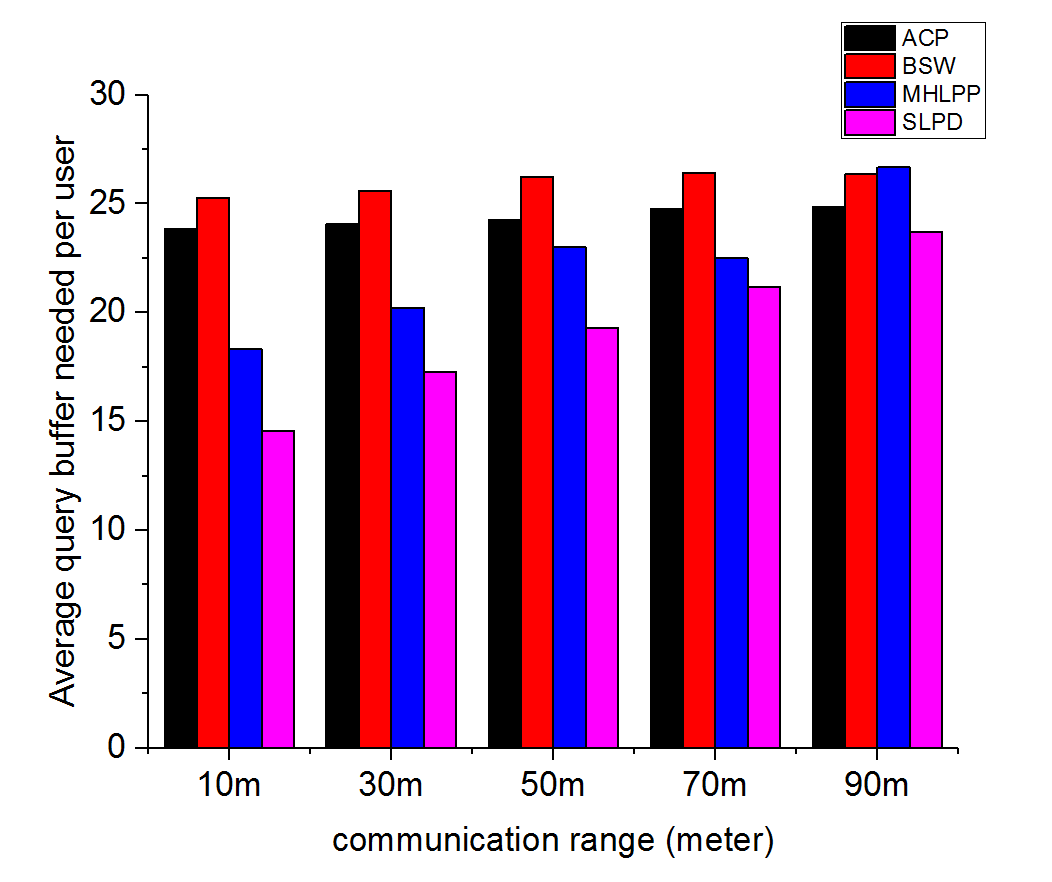
\includegraphics[width=4.0in]{olgraph/QbnpuCr.png}
\caption{Average Number of Query Buffer Needed at 20 Minutes Mark} 
\label{fig:F419AverageQueryBufferNeededAt20Minutes} %% label for entire figure 
\end{figure}

The Figure \ref{fig:F420AverageNumberofCarriedQueriesPerUser} shows the average number of queries which are carried by users in communication ranges 10, 50 and 90 meters. The curves for ACP and BSW rise sharply at the beginning and then become flat, while those for MHLPP and SLPD rise smoothly and continuously. 

\begin{figure} [hbtp]
\centering 
\subfigure[communication range is equal to 10 meters]{ 
\label{fig:F420AverageNumberofCarriedQueriesPerUser:a} %% label for first subfigure 
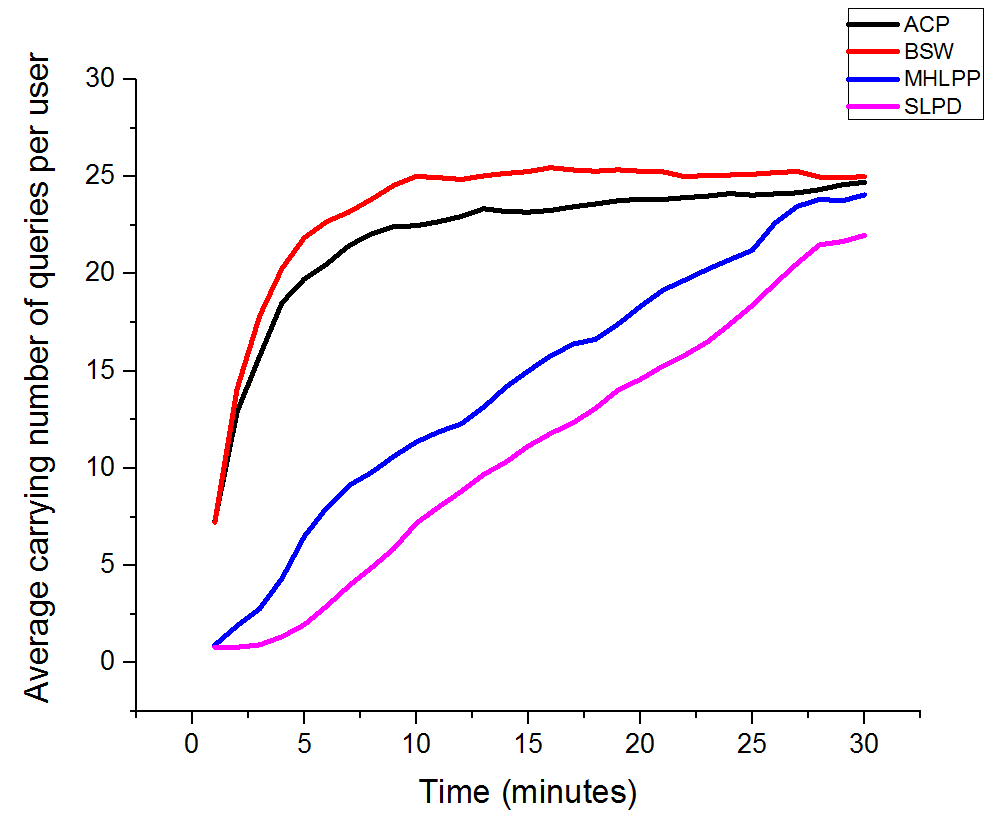
\includegraphics[width=3.0in]{figures/F420AverageNumberofCarriedQueriesPerUser10.png}} 
\hspace{1in} 
\subfigure[communication range is equal to 50 meters]{ 
\label{fig:AverageNumberofCarriedQueriesPerUser:b} %% label for second subfigure 
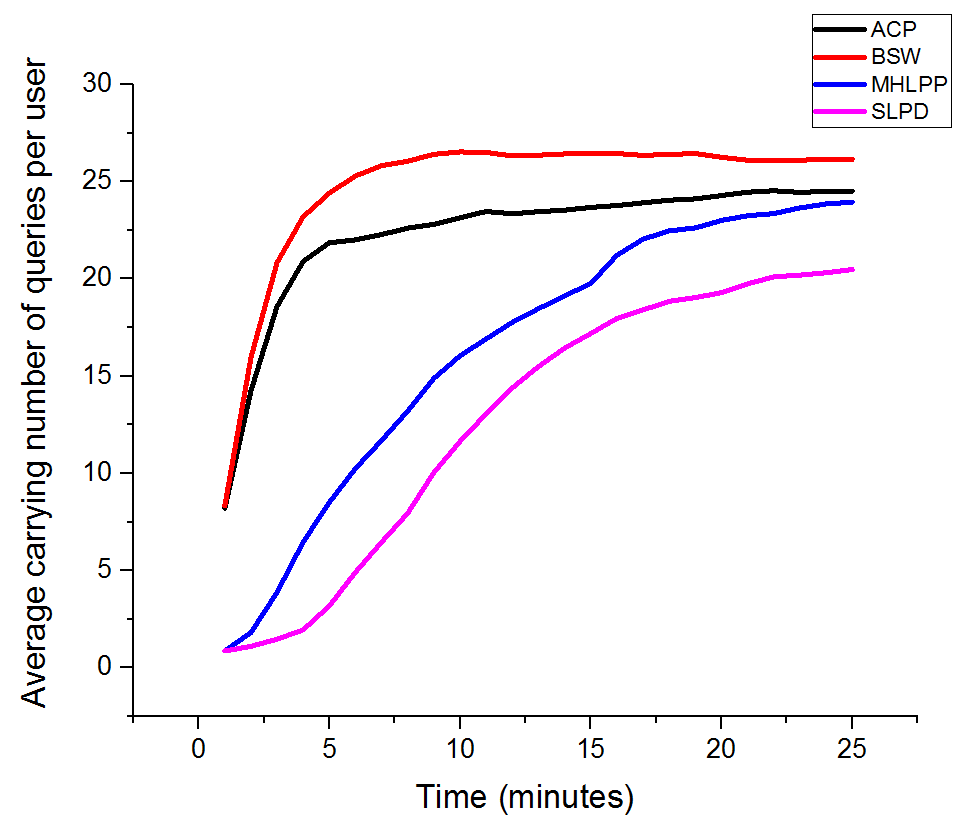
\includegraphics[width=3.0in]{figures/F420AverageNumberofCarriedQueriesPerUser50.png}}
\hspace{1in} 
\subfigure[communication range is equal to 90 meters]{ 
\label{fig:AverageNumberofCarriedQueriesPerUser:c} %% label for second subfigure 
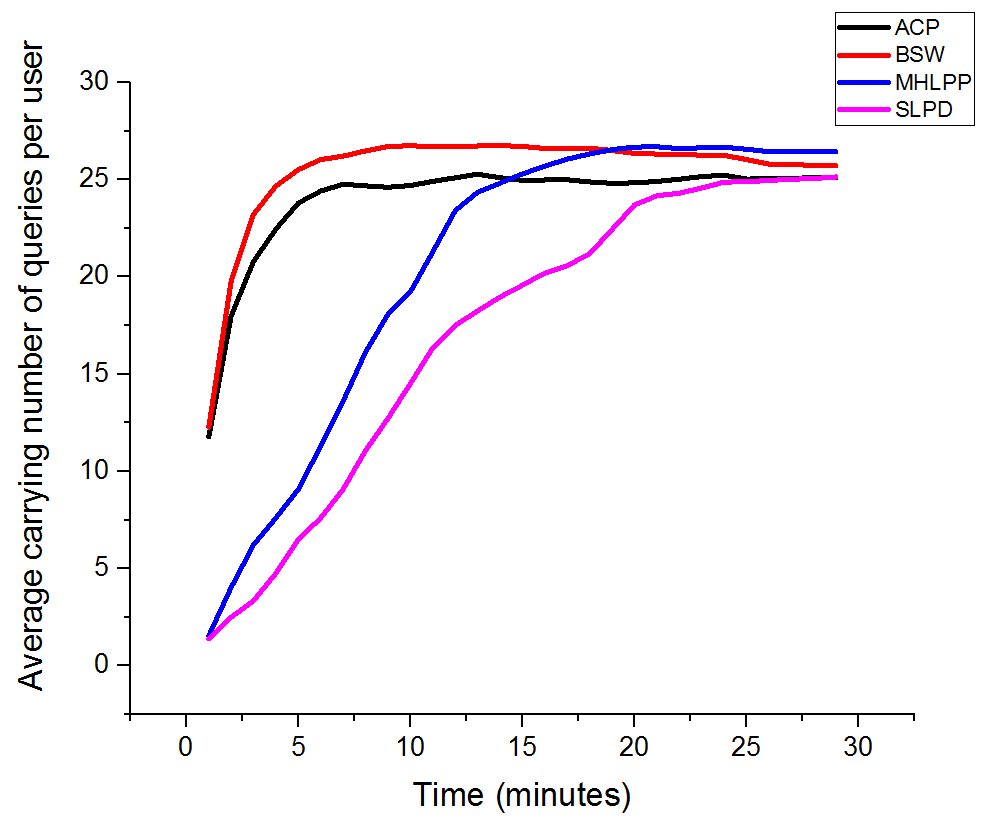
\includegraphics[width=3.0in]{figures/F420AverageNumberofCarriedQueriesPerUser90.png}}
\caption{Average Number of Queries Carried Per User} 
\label{fig:F420AverageNumberofCarriedQueriesPerUser} %% label for entire figure 
\end{figure}

\subsection{ Distributing Appointment Cards}

\noindent Exchanging ACs is a feature of proposed ACP, which can be considered as an extra cost. We count the number of exchanging ACs per minute to evaluate this extra cost of ACP.

In Figure \ref{fig:F422AverageNumberofExchangingACsPerMinute}, we show the total number of exchanging ACs in the whole network. For example, if an user Alice encounters another user Bob, the total number of exchanging ACs processes increases by one when Alice exchanges any ACs to Bob. We count the number of those exchanging processes occur per minute. As shown in the figure \ref{fig:F422AverageNumberofExchangingACsPerMinute}, the exchanging processes do not occur frequently, but about 2 times per minutes. Since the size of an AC is small, it does not consume too much network resource. At the same time, users can get many ACs to help them send queries, as shown in Figure \ref{fig:F421AverageNumberofReadyACsPerUser}. The number of ready ACs per user is raising smoothly and steadily. 

\begin{figure} [hbtp]
\centering 
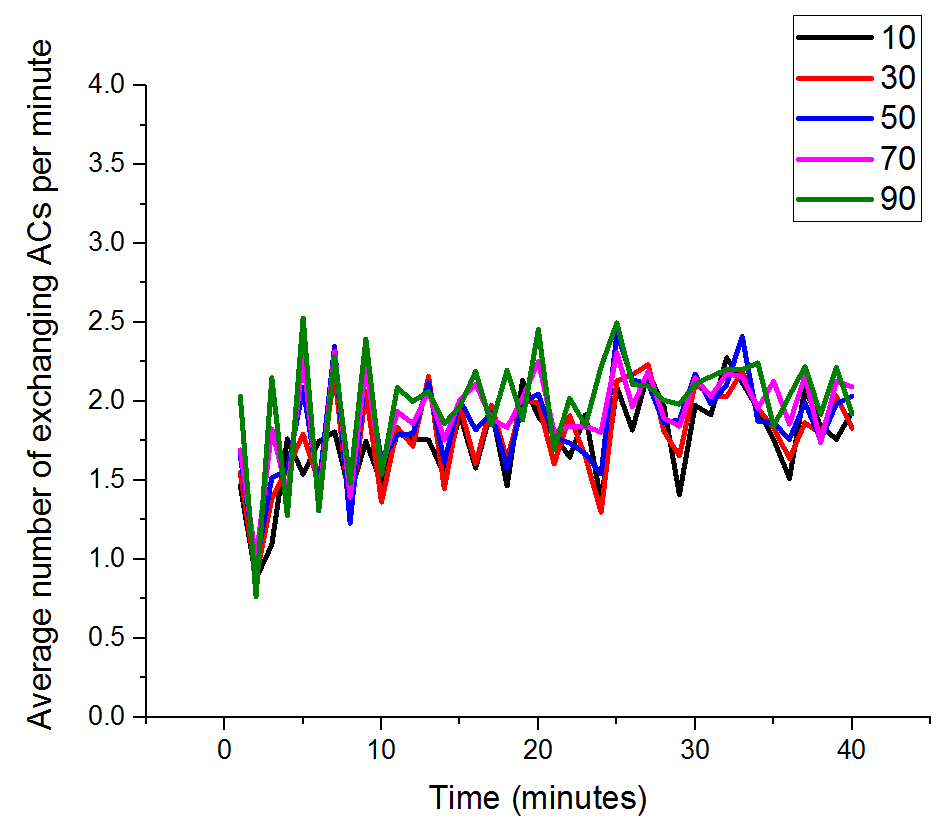
\includegraphics[width=4.0in]{figures/F422AverageNumberofExchangingACsPerMinute.png}
\caption{Average Number of Exchanging ACs Per Minute Under Different Communication Ranges} 
\label{fig:F422AverageNumberofExchangingACsPerMinute} %% label for entire figure 
\end{figure}

\begin{figure} [hbtp]
\centering 
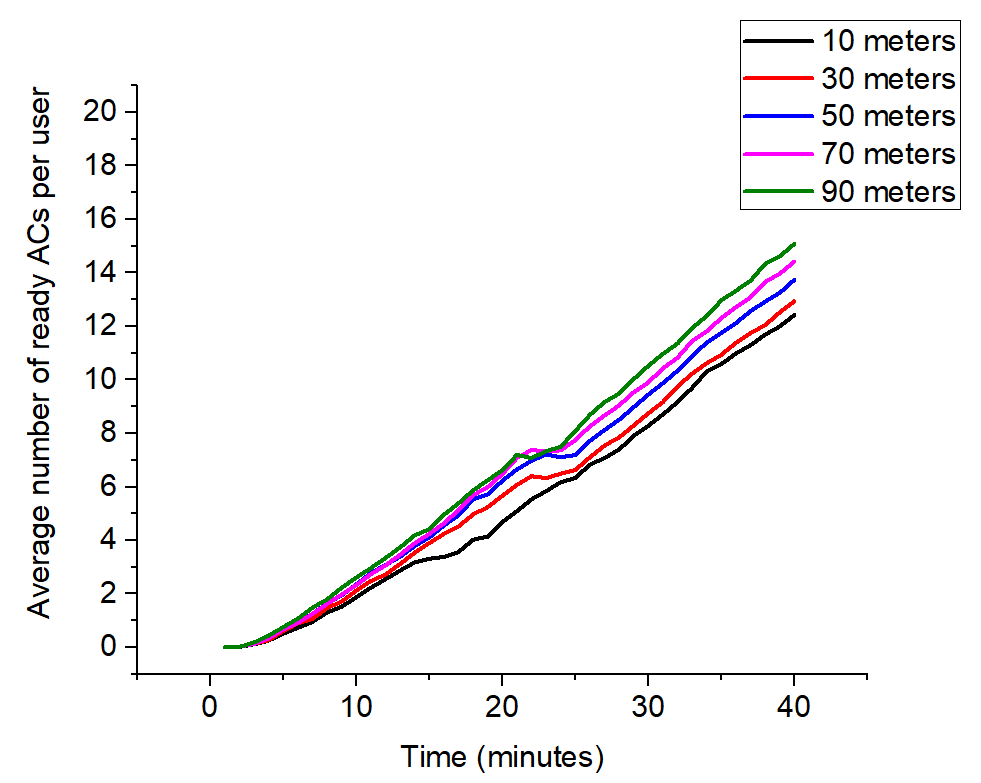
\includegraphics[width=4.0in]{figures/F421AverageNumberofReadyACsPerUser.png}
\caption{Average Number of Ready ACs Per User} 
\label{fig:F421AverageNumberofReadyACsPerUser} %% label for entire figure 
\end{figure}



